\filbreak
\subsection*{\texorpdfstring{سؤال $1$ امتحان $\mathrm{899371}$ سنة $2025$}{سؤال 1 امتحان 899371 سنة 2025}}
\phantomsection
\addcontentsline{toc}{subsection}{\texorpdfstring{سؤال $1$ امتحان $\mathrm{899371}$ سنة $2025$}{سؤال 1 امتحان 899371 سنة 2025}}

\noindent
\makebox[\textwidth][c]{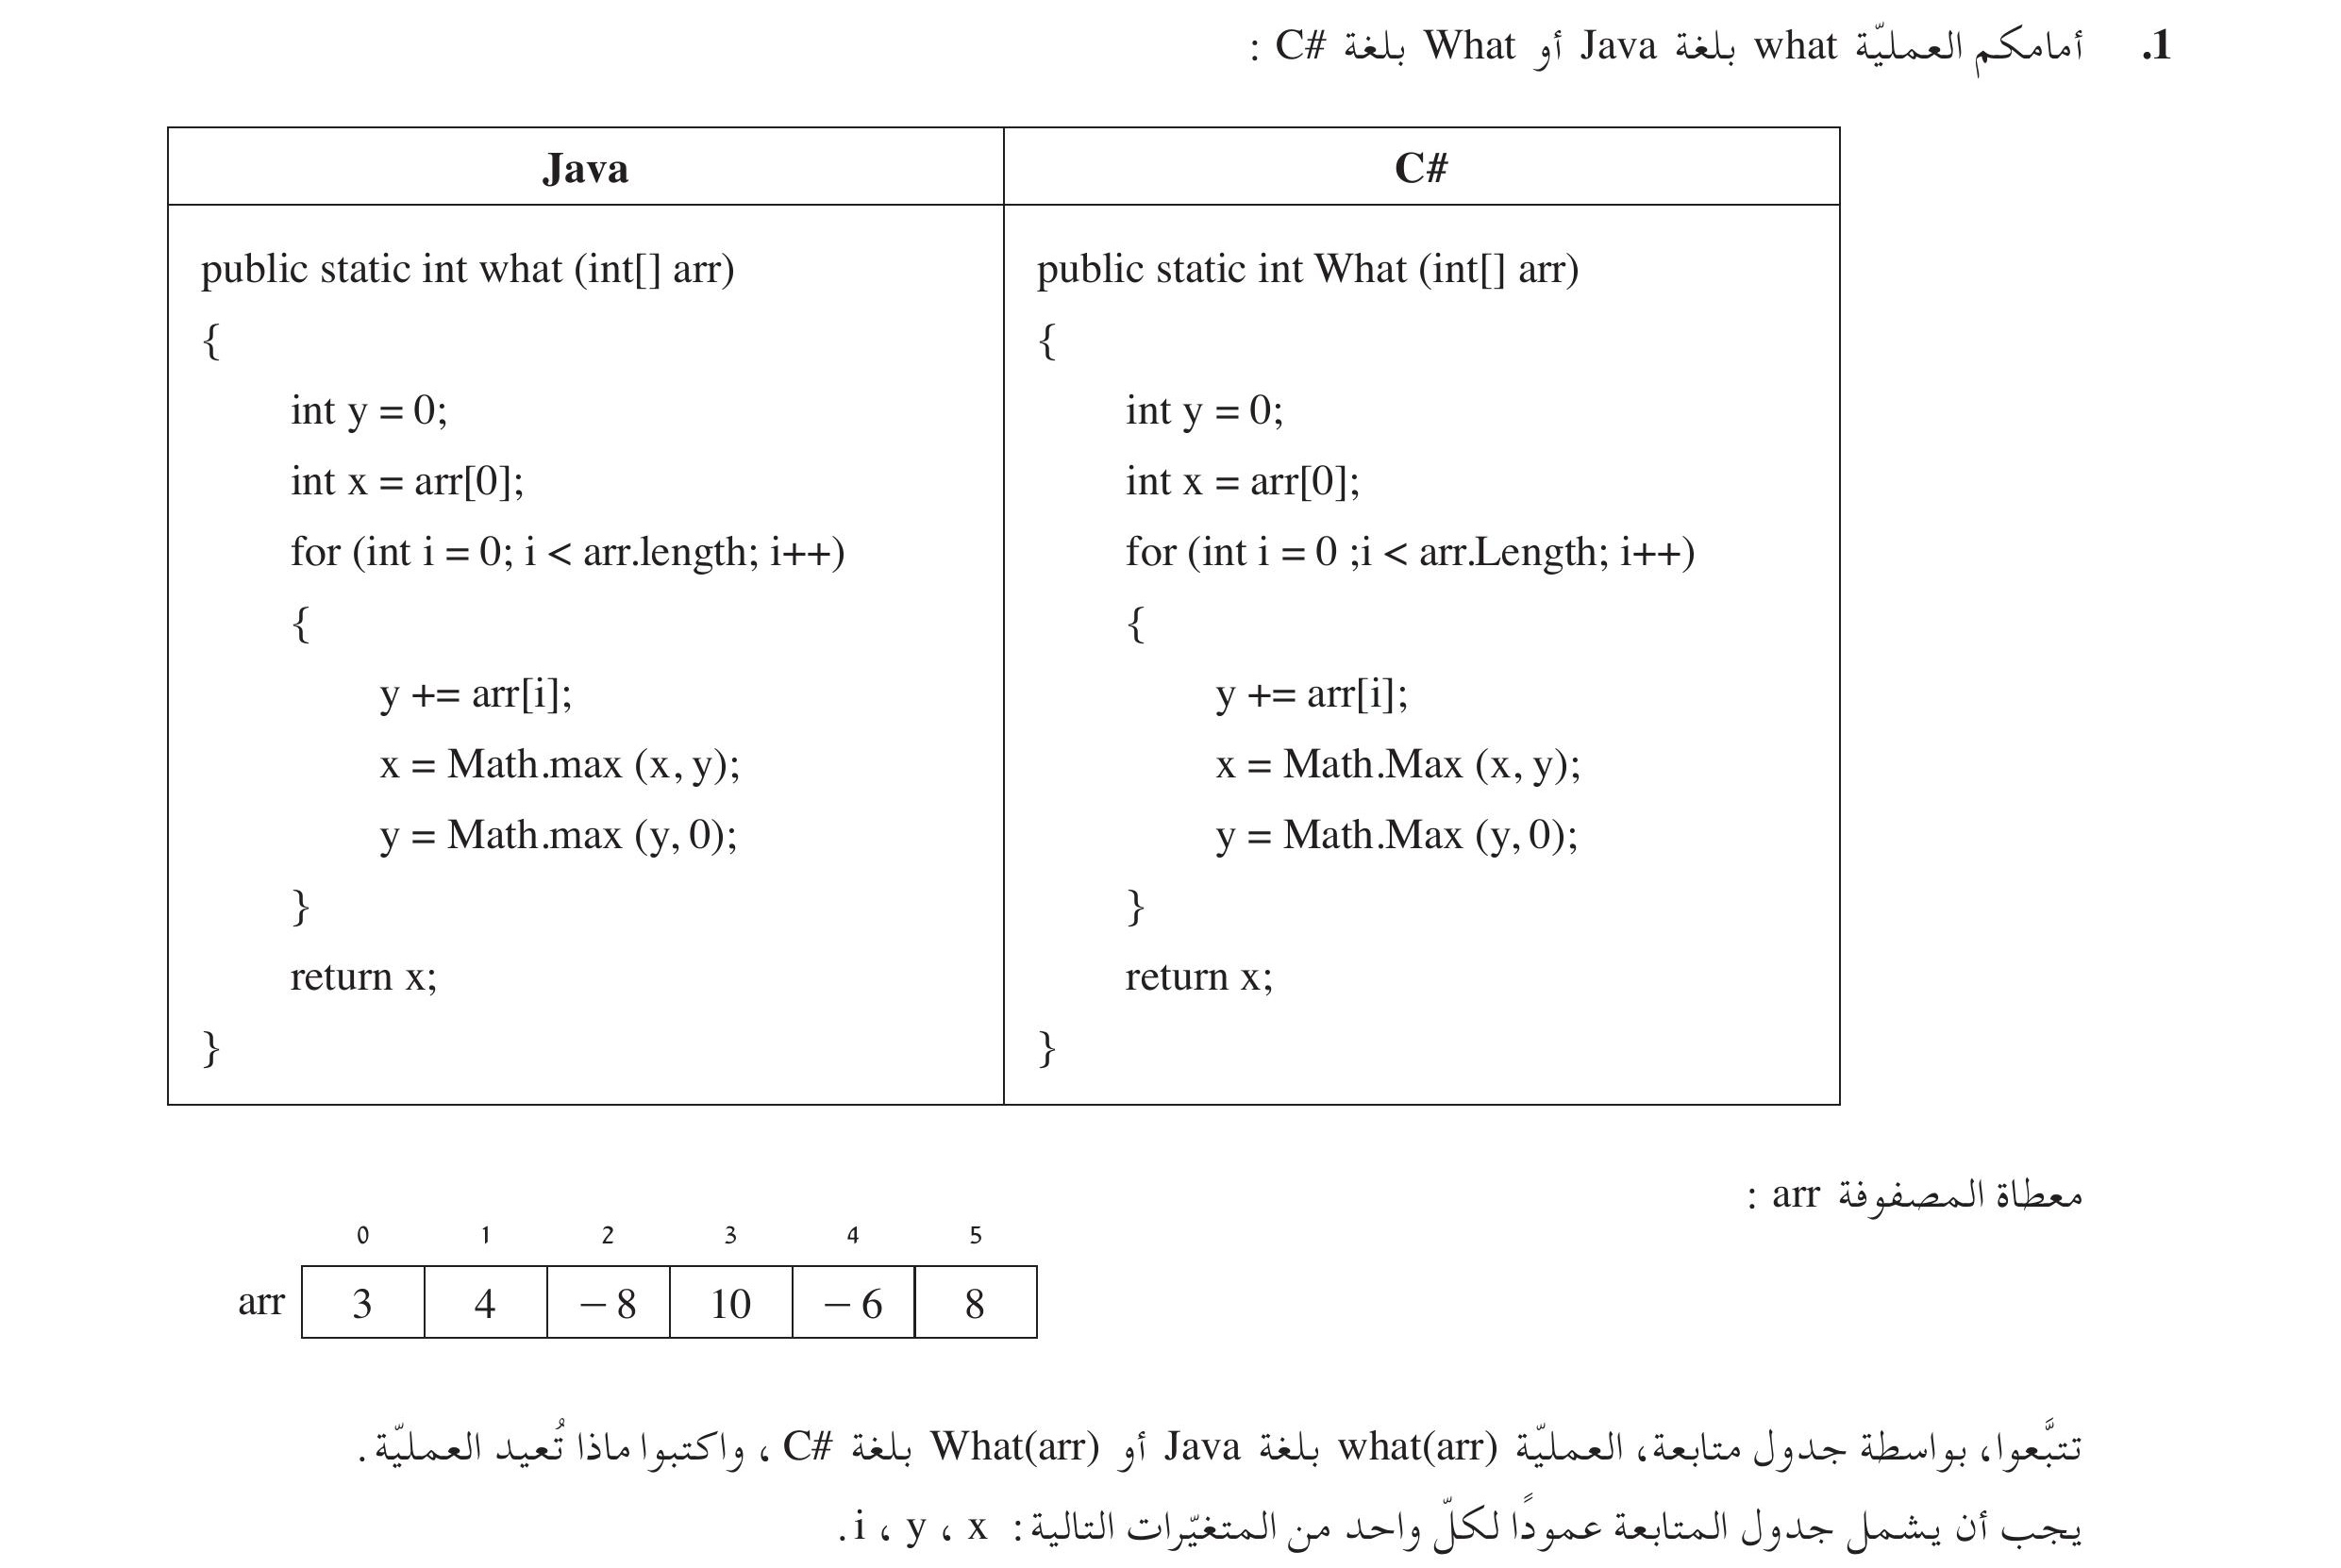
\includegraphics[width=0.9\paperwidth,keepaspectratio]{ ../../../bagrut_questions/basics/arrays_2025_899371_1.jpg }%
}%


% \ifwithsols
% \begin{boxSolution}[\texorpdfstring{سؤال $1$ امتحان $\mathrm{899371}$ سنة $2025$}{سؤال 1 امتحان 899371 سنة 2025}]
% \begin{enumerate}[itemsep=1.5em, label=\alph*.]
%     \item .
% \begin{boxCode}
% \begin{english}
% \begin{minted}{csharp}
% // TODO
% \end{minted}
% \end{english}
% \end{boxCode}
% \end{enumerate}
% \end{boxSolution}
% \fi
\filbreak
